%%%%%%%%%%%%%%%%%%%%%%%%%%%%%%%%%%%%%%%%%
% Wenneker Article
% LaTeX Template
% Version 2.0 (28/2/17)
%
% This template was downloaded from:
% http://www.LaTeXTemplates.com
%
% Authors:
% Vel (vel@LaTeXTemplates.com)
% Frits Wenneker
%
% License:
% CC BY-NC-SA 3.0 (http://creativecommons.org/licenses/by-nc-sa/3.0/)
%
%%%%%%%%%%%%%%%%%%%%%%%%%%%%%%%%%%%%%%%%%

%----------------------------------------------------------------------------------------
%	PACKAGES AND OTHER DOCUMENT CONFIGURATIONS
%----------------------------------------------------------------------------------------

\documentclass[12pt, a4paper, twocolumn]{article} % 10pt font size (11 and 12 also possible), A4 paper (letterpaper for US letter) and two column layout (remove for one column)

\usepackage[utf8]{inputenc}
\usepackage[italian]{babel}
\usepackage{float}
\usepackage{wrapfig}
\setcounter{tocdepth}{0}

%%%%%%%%%%%%%%%%%%%%%%%%%%%%%%%%%%%%%%%%%
% Wenneker Article
% Structure Specification File
% Version 1.0 (28/2/17)
%
% This file originates from:
% http://www.LaTeXTemplates.com
%
% Authors:
% Frits Wenneker
% Vel (vel@LaTeXTemplates.com)
%
% License:
% CC BY-NC-SA 3.0 (http://creativecommons.org/licenses/by-nc-sa/3.0/)
%
%%%%%%%%%%%%%%%%%%%%%%%%%%%%%%%%%%%%%%%%%

%----------------------------------------------------------------------------------------
%	PACKAGES AND OTHER DOCUMENT CONFIGURATIONS
%----------------------------------------------------------------------------------------

\usepackage[italian]{babel} % English language hyphenation

\usepackage{microtype} % Better typography

\usepackage{amsmath,amsfonts,amsthm} % Math packages for equations

\usepackage[svgnames]{xcolor} % Enabling colors by their 'svgnames'

\usepackage[hang, small, labelfont=bf, up, textfont=it]{caption} % Custom captions under/above tables and figures

\usepackage{booktabs} % Horizontal rules in tables

\usepackage{lastpage} % Used to determine the number of pages in the document (for "Page X of Total")

\usepackage{graphicx} % Required for adding images

\usepackage{enumitem} % Required for customising lists
\setlist{noitemsep} % Remove spacing between bullet/numbered list elements

\usepackage{sectsty} % Enables custom section titles
\allsectionsfont{\usefont{OT1}{phv}{b}{n}} % Change the font of all section commands (Helvetica)

%----------------------------------------------------------------------------------------
%	MARGINS AND SPACING
%----------------------------------------------------------------------------------------

\usepackage{geometry} % Required for adjusting page dimensions

\geometry{
	top=1cm, % Top margin
	bottom=1.5cm, % Bottom margin
	left=2cm, % Left margin
	right=2cm, % Right margin
	includehead, % Include space for a header
	includefoot, % Include space for a footer
	%showframe, % Uncomment to show how the type block is set on the page
}

\setlength{\columnsep}{7mm} % Column separation width

%----------------------------------------------------------------------------------------
%	FONTS
%----------------------------------------------------------------------------------------

\usepackage[T1]{fontenc} % Output font encoding for international characters
\usepackage[utf8]{inputenc} % Required for inputting international characters

\usepackage{XCharter} % Use the XCharter font

%----------------------------------------------------------------------------------------
%	HEADERS AND FOOTERS
%----------------------------------------------------------------------------------------

\usepackage{fancyhdr} % Needed to define custom headers/footers
\pagestyle{fancy} % Enables the custom headers/footers

\renewcommand{\headrulewidth}{0.0pt} % No header rule
\renewcommand{\footrulewidth}{0.4pt} % Thin footer rule

\renewcommand{\sectionmark}[1]{\markboth{#1}{}} % Removes the section number from the header when \leftmark is used

%\nouppercase\leftmark % Add this to one of the lines below if you want a section title in the header/footer

% Headers
\lhead{} % Left header
\chead{\textit{\thetitle}} % Center header - currently printing the article title
\rhead{} % Right header

% Footers
\lfoot{} % Left footer
\cfoot{} % Center footer
\rfoot{\footnotesize Page \thepage\ of \pageref{LastPage}} % Right footer, "Page 1 of 2"

\fancypagestyle{firstpage}{ % Page style for the first page with the title
	\fancyhf{}
	\renewcommand{\footrulewidth}{0pt} % Suppress footer rule
}

%----------------------------------------------------------------------------------------
%	TITLE SECTION
%----------------------------------------------------------------------------------------

\newcommand{\authorstyle}[1]{{\large\usefont{OT1}{phv}{b}{n}\color{DarkRed}#1}} % Authors style (Helvetica)

\newcommand{\institution}[1]{{\footnotesize\usefont{OT1}{phv}{m}{sl}\color{Black}#1}} % Institutions style (Helvetica)

\usepackage{titling} % Allows custom title configuration

\newcommand{\HorRule}{\color{DarkGoldenrod}\rule{\linewidth}{1pt}} % Defines the gold horizontal rule around the title

\pretitle{
	\vspace{-30pt} % Move the entire title section up
	\HorRule\vspace{10pt} % Horizontal rule before the title
	\fontsize{32}{36}\usefont{OT1}{phv}{b}{n}\selectfont % Helvetica
	\color{DarkRed} % Text colour for the title and author(s)
}

\posttitle{\par\vskip 15pt} % Whitespace under the title

\preauthor{} % Anything that will appear before \author is printed

\postauthor{ % Anything that will appear after \author is printed
	\vspace{10pt} % Space before the rule
	\par\HorRule % Horizontal rule after the title
	\vspace{20pt} % Space after the title section
}

%----------------------------------------------------------------------------------------
%	ABSTRACT
%----------------------------------------------------------------------------------------

\usepackage{lettrine} % Package to accentuate the first letter of the text (lettrine)
\usepackage{fix-cm}	% Fixes the height of the lettrine

\newcommand{\initial}[1]{ % Defines the command and style for the lettrine
	\lettrine[lines=3,findent=4pt,nindent=0pt]{% Lettrine takes up 3 lines, the text to the right of it is indented 4pt and further indenting of lines 2+ is stopped
		\color{DarkGoldenrod}% Lettrine colour
		{#1}% The letter
	}{}%
}

\usepackage{xstring} % Required for string manipulation

\newcommand{\lettrineabstract}[1]{
	\StrLeft{#1}{1}[\firstletter] % Capture the first letter of the abstract for the lettrine
	\initial{\firstletter}\textbf{\StrGobbleLeft{#1}{1}} % Print the abstract with the first letter as a lettrine and the rest in bold
}

%----------------------------------------------------------------------------------------
%	BIBLIOGRAPHY
%----------------------------------------------------------------------------------------

% \usepackage[backend=bibtex,style=authoryear,natbib=true]{biblatex} % Use the bibtex backend with the authoryear citation style (which resembles APA)

\addbibresource{example.bib} % The filename of the bibliography

\usepackage[autostyle=true]{csquotes} % Required to generate language-dependent quotes in the bibliography
 % Specifies the document structure and loads requires packages

% \usepackage{textcomp}
%----------------------------------------------------------------------------------------
%	ARTICLE INFORMATION
%----------------------------------------------------------------------------------------

\title{Sound of Data} % The article title

\author{
  \authorstyle{
    % DO NOT TOUCH HSPACEs!! @Momo
    Riccardo Cervero \hspace{25pt} 794126 \\  % x + 4
    Marco Ferrario \hspace{44pt}  795203 \\   % x + 23
    Pranav Kasela \hspace{46.5pt} 846965 \\   % x + 25.5
    Federico Moiraghi \hspace{21pt} 799735    % x
  } % Authors
  \newline\newline
  \institution{Università degli Studi di Milano Bicocca}
}

\date{Anno Accademico 2018/19} % Add a date here if you would like one to appear underneath the title block, use \today for the current date, leave empty for no date

%----------------------------------------------------------------------------------------

\begin{document}

\maketitle % Print the title

\thispagestyle{firstpage} % Apply the page style for the first page (no headers and footers)

%----------------------------------------------------------------------------------------
%	ABSTRACT
%----------------------------------------------------------------------------------------

\lettrineabstract{Obiettivo del progetto è analizzare la discussione mediatica sul social network Twitter studiando in tempo reale l'andamento della discussione nell'ambito musicale, presente e passato, per verificare la presenza di variazioni all'interno del ciclo giornaliero e la presenza di comunità digitali e le loro interconnessioni.
Il presente lavoro può essere di aiuto nella costruzione di sistemi di raccomandazione interni a Twitter (quali pagine consigliate) e nella programmazione di BOT, a scopo pubblicitario, che intendano infilarsi in una discussione mediatica già presente (ovvero argomenti di tendenza) per inserire i propri messaggi.}
\newpage

\tableofcontents
\hfill
\newpage

%----------------------------------------------------------------------------------------
%	ARTICLE CONTENTS
%----------------------------------------------------------------------------------------
\part{Introduzione}
I traguardi posti dal progetto \textit{Sound of Data}\footnote{\url{https://github.com/pkasela/Sound-of-Data}}, hanno innanzitutto richiesto l'uso di uno \textit{knowledge graph} adeguato alla materia: scaricato un \textit{dump} di \url{musicbrainz.org}, versione \textit{semantic web} di \url{last.fm}, disponibile pubblicamente in formato \verb|.tsv| (\textit{Tabular Separated Values}), si è provveduto ad importarlo all'interno di Apache Hadoop\footnote{\url{https://hadoop.apache.org}} per effettuare una rapida pulizia preliminare.
Fatto ciò, i dati sono stati importati in Neo4J\footnote{\url{https://neo4j.com}}, grazie al pratico programma \verb|neo4j-import|, in modo da costruire lo \textit{knowledge graph} richiesto per l'analisi dei \textit{tweet}, raccolti ed analizzati in tempo reale grazie ad Apache Kafka\footnote{\url{https://kafka.apache.org}}: grazie ad un efficiente plug-in che permette l'uso di \textit{Neo4j} come \textit{Consumer}, il singolo tweet è archiviato nativamente in uno schema a grafo.
Durante il processo di \textit{streaming}, questi subiscono varie operazioni di \textit{preparation} e vengono filtrati da un rudimentale strumento di \textit{instance matching}.

Dopo la complessa fase di gestione e raccolta dei dati, è stato possibile condurre un'analisi finale sulle dinamiche della discussione musicale instauratesi fra i singoli utenti all'interno di comunità, astratte ed estremamente mutevoli, e sulle relazioni, più o meno intense, esistenti fra di esse.
Le progressiva composizione che i nodi associati ai \textit{tweet} assumono all'interno del grafo è studiata ad intervalli più o meno regolari, corrispondenti a quattro fasce orarie relative al mattino, pomeriggio, sera, notte.
Si è preferito adoperare tale ciclo giornaliero, anziché un più ampio ciclo settimanale, o addirittura mensile, per due ragioni precise.
Innanzitutto, questo garantisce una più facile interpretazione: risulta di estremo interesse osservare i trend ricorrenti nei vari momenti della giornata, piuttosto che riferiti all'arco settimanale.
Inoltre, il ciclo giornaliero ha il vantaggio di non risentire della distorsione provocata dagli eventi, previsti o meno.
Infatti, essendo gli eventi in grado di assorbire l'interesse della gran parte dell'opinione pubblica per interi giorni e settimane, questi penalizzano l'analisi e concentrano tutti gli utenti verso un numero limitato di argomenti musicali.
Due esempi riguardanti tale problematica, e le sue conseguenze negative, possono essere citati per quanto concerne il genere \textit{drone}, per cui durante il periodo di raccolta, si sono succeduti due eventi particolarmente rilevanti: il primo riguarda l'abbattimento di un drone americano in territorio Iraniano, causando nuove tensioni fra i due Paesi\footnote{\url{http://www.ansa.it/sito/notizie/mondo/mediooriente/2019/06/20/iran-pasdaran-abbattuto-drone-usa_b8922ea0-e61c-436b-8f66-60f3be32ed21.html}}, mentre il secondo consiste in uno spettacolo di droni luminosi a Torino\footnote{\url{https://www.guidatorino.com/eventi-torino/san-giovanni-torino-droni-2019/}} per la festa patronale.

Raccogliendo l'attenzione di centinaia di utenti, i due eventi e la polisemia della parola hanno fatto sì che la comunità di ascoltanti il genere musicale \textit{drone} fosse sproporzionatamente più grande rispetto alle altre nei giorni degli eventi; ma tale distorsione è diluita dalla divisione in fasce orarie e dalla moltitudine dei giorni in cui è stata effettuata la raccolta dati.
\hfill
\newpage


\part{Costruzione dello \textit{knowledge graph}}

\section{Data Cleaning con Python e Pig}
%Riferimenti `Bibliografici'
%https://www.infoq.com/articles/apache-tez-saha-murthy/
%https://tez.apache.org/


I dati sono scaricati dal sito di musicbrainz attraverso lo script python \verb|get_data.py|\footnote{\url{https://github.com/pkasela/Sound-of-Data/blob/master/musicbrainz_data/Data_Cleaning/get_data.py}} che cerca sul sito l'ultima versione del database e la scarica col comando \verb|wget| dei sistemi Unix.
Decompressa quindi la cartella compressa con il dump del database e selezionati solamente i file necessari allo scopo, sono eseguite delle operazioni \verb|cat-sed| per effettuare una rapida pulizia preliminare (la gestione dei valori nulli \verb|\N|).
È salvata inoltre una lista di generi musicali, già presente in una pagina HTML del sito, tramite uno \textit{scraper}, che ne analizza l'elenco per importarla in Python.

%%%%%%
%%%%%%%%%%%
%%%%%%%%%%%%%%%%
%%%% Ma lo schema iniziale va messo?
%%%% Io dico di no al massimo lo schema finale
%%%%%%%%%%%%%%%%
%%%%%%%%%%%
%%%%%%

I file sono successivamente importati e processati all'interno del \textit{file system} HDFS.
Nel dettaglio, questa fase viene eseguita attraverso l'utilizzo di Apache Pig, piattaforma atta all'elaborazione di grosse quantità di dati.
La decisione di utilizzare Pig anzichè SQL dipende principalmente dalle migliori prestazioni del primo nella fase di caricamento, e dalla maggiore versatilità della suite Hadoop per la fase di elaborazione.
L'\textit{engine} adoperato in combinazione con Pig non è MapReduce ma Tez: costruito sopra YARN, migliora drasticamente le prestazioni mantenendo la stessa scalabilità evitando alcune fasi di scrittura di risultati parziali sull'HDFS (vedere Figura \ref{fig:Hadoop} per maggiori dettagli).

\begin{figure*}
  \centering
  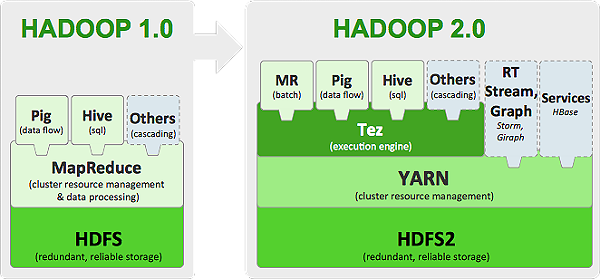
\includegraphics[width=\linewidth]{hadoop2.png}
  \caption{Differenza architteturale di HADOOP 1.0 con MapReduce rispetto alla versione 2.0 con Tez.}
  \label{fig:Hadoop}
\end{figure*}

Più precisamente, la velocità di esecuzione è ottenuta grazie all'invio diretto dei dati da un processo all'altro, evitando la scrittura all'interno del file system, eccezion fatta per i \textit{checkpoints}.
Inoltre, la definizione del \textit{job} sfrutta i \textit{Directed Acyclic Graph}, dove i vertici rappresentano gli step del processo e gli archi la connessione tra i vertici \textit{Producer} e \textit{Consumer} (come mostrato in Figura \ref{fig:Tez}).

\begin{figure*}
  \centering
  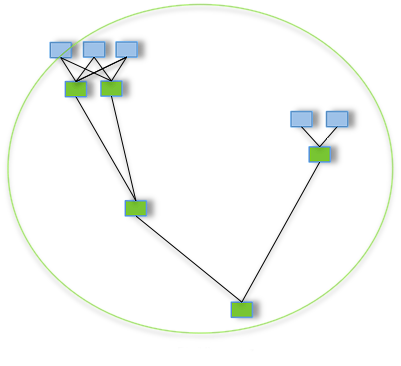
\includegraphics[width=0.9\linewidth]{tez.png}
  \caption{Funzionamento di Tez.}
  \label{fig:Tez}
\end{figure*}

Conclusa la fase di pulizia, i dati sono trasferiti all'esterno di HDFS, sul filesystem reale, unendo i risultati di Pig  mediante il comando \textit{cat} di \textit{Unix}. 
A questo punto i dati sono pronti per essere importati in Neo4j.

%%%%%%
%%%%%%%%%%%
%%%%%%%%%%%%%%%%
%%%% Conviene mettere lo schema finale delle tabelle (dopo lo metto)
%%%%%%%%%%%%%%%%
%%%%%%%%%%%
%%%%%%

\section{Import dei dati in Neo4J}
%Reference
%https://neo4j.com/docs/operations-manual/current/tutorial/import-tool/
Infine, il risultato dell'elaborazione svolta da Pig viene caricato all'interno del \textit{DBMS Neo4j}, usando il comando \verb|neo4j-import|, indicizzando i \textit{gid} delle varie entità, in modo da velocizzare la ricerca da svolgere successivamente.
%cosa altro si deve scrivere hahaha

Il risultato è un grafo dal peso approssimativo di 5Gb contenente i vari artisti, i relativi album e le relative case discografiche collegate in modo opportuno.
Si è preferito ridurre la capillarità del database non inserendo le singole canzoni contenute negli album, sia perché una simile precisione sarebbe stata difficile da gestire in fase di analisi, sia a causa della mancanza nel dump del database di tale informazione (comunque presente nella versione online), che avrebbe richiesto un tempo superiore alla settimana (dovuto perlopiù alla latenza supportata dal sito) per poter essere recuperata.


\hfill
\newpage
\part{Analisi dei tweet}
\section{Elaborazione mediante Apache Kafka}
%Reference 
%https://github.com/neo4j-contrib/neo4j-streams
%https://riak-python-client.readthedocs.io/en/1.5-stable/tutorial.html
Nella fase di gestione e analisi in tempo reale, i \textit{tweet} sono filtrati ed elaborati mediante una sequenza di operazioni, attraverso una \textit{pipeline} costituita dalla concatenazione di due coppie di processi Producer e Consumer.
L'architettura di elaborazione in \textit{streaming} è stata così configurata per garantire una maggiore scalabilità ed una migliore performance, riuscendo a reggere maggiori volumi di \textit{tweet} in ingresso.
Questi vengono estratti grazie all'API \textit{Tweepy}\footnote{\url{https://tweepy.readthedocs.io/en/latest/}} per Python, utilizzando come parole chiave di ricerca una selezione di 400 generi musicali fra i 419 ottenuti dallo scraping della pagina \url{'https://musicbrainz.org/genres'}, e ricevendo soltanto i testi pubblicati in lingua italiana.

Quindi sono inviati ad una prima Topic come messaggi di un \textit{Producer} di Kafka, inizializzato mediante la libreria \textit{Kafka-python}\footnote{\url{https://kafka-python.readthedocs.io/en/master/}}. 
All'interno di un secondo file\footnote{\url{https://github.com/pkasela/Sound-of-Data/blob/master/NL/Kafka_Producer_2.py}}, associato ad un nuovo processo Producer, dunque ad una seconda Topic connessa in \textit{streaming} con la precedente, il JSON grezzo che costituisce ciascun \textit{tweet} in ingresso viene processato in vari step dalla funzione \verb|tweet_preparations|.

La prima fase coincide con l'estrazione dello \textit{screen name} dell'utente, del contenuto postato e dell'ora e data precisa di pubblicazione. 
In particolare, il testo viene modificato in modo da rendere leggibili i caratteri speciali e i cosiddetti \textit{escape characters}. 

La seconda fase sfrutta l'API di \textit{Botometer}\footnote{\url{https://rapidapi.com/OSoMe/api/botometer/details}} per calcolare la probabilità - definita \textit{score} - che un profilo sia in realtà gestito da un BOT, osservandone il comportamento passato.
Poiché i profili gestiti in modo automatico alterano, spesso fortemente, la discussione mediatica aumentando arbitrariamente il flusso di determinati contenuti, si è deciso di non archiviare i \textit{tweet} appartenenti a tali profili. 
Nel dettaglio, se lo score associato all'utente di ogni \textit{tweet} supera una soglia (fissata arbitrariamente al $90\%$), lo \textit{screen name} viene memorizzato all'interno di una \textit{blacklist}, altrimenti smistato in una \textit{whitelist}, in modo che il programma possa riconoscere più velocemente ogni profilo ed evitare inutili ricalcoli e così da ridurre il numero di richieste fatte all'API, gratuita fino ad un certo volume e poi a pagamento.
Per aumentare ulteriormente l'efficienza di questo processo e garantire la scalabilità, si è scelto di adoperare il \textit{data store Riak}, di tipo \textit{NoSQL Key-Value}, attraverso la propria libreria in Python\footnote{\url{https://github.com/basho/riak-python-client}}: è così archiviato lo \textit{score} di ogni utente e la richiesta all'API è effettuata solamente se non è trovata la chiave nel database.

La terza fase verifica che il testo sia effettivamente legato al tema musicale grazie ad un rudimentale \textit{istance matcher} che tenta di riconoscere le parole riguardanti il contesto musicale, aggiungendo al dizionario prodotto dalle fasi precedenti tre chiavi corrispondenti rispettivamente alla lista di artisti, album o canzoni estratti dal testo analizzato.
Ciò è permesso dall'uso dell'API\footnote{\url{https://python-musicbrainzngs.readthedocs.io/en/v0.6/api/}} fornita dal sito \textit{musicbrainz.org} e basata su Apache Lucene\footnote{\url{https://lucene.apache.org/}}.
Per maggiori dettagli si rimanda alla sezione dedicata.

Ogniqualvolta si verificano le due condizioni note, cioè che l'utente non abbia probabilità elevata di essere un BOT e che il testo pubblicato si riferisca effettivamente al mondo della musica, ciascun risultato della funzione \verb|tweet_preparations| è ricodificato e passato come messaggio al secondo \textit{Producer} di \textit{Apache Kafka} - menzionato in precedenza - che effettuerà l'invio del dato finale alla \textit{topic} nominata \textit{KafkaTopic}. 
Grazie all'utilizzo di questa piattaforma, il flusso di \textit{feed} è gestito in tempo reale, assicurando bassissima latenza e grande scalabilità. 

\section{Consuming dei Tweets in Neo4j}
Un principale vantaggio di \textit{Apache Kafka} consiste nella capacità di connettersi efficientemente a sistemi esterni, garantendo in tal modo la continuità dello \textit{stream} di dati da una fonte - la class \textit{Listener} adoperata in Python per "ascoltare" i tweet grazie all'API Tweepy - ad una \textit{"landing zone"}, che in questo caso corrisponde al DBMS \textit{Neo4j}. 
Si è scelto di effettuare lo \textit{storage} dei tweets in un \textit{GraphDB}, e in particolare \textit{Neo4j}, tra le varie motivazioni, per le sue caratteristiche di estrema scalabilità, efficienza nella gestione dei dati, elevata capacità di adattamento al fenomeno di studio e facile interpretabilità.
L'esportazione diretta dei tweet da \textit{Apache Kafka} all'interno del \textit{data store} avviene grazie a un \textit{plug-in} di \textit{Neo4j}, \textit{"Neo4j Streams Consumer"}. Questo si configura come un'applicazione che effettua un'ingestione diretta e automatizzata all'interno di \textit{Neo4j}, permettendo la lettura dei dati presenti nella \textit{topic} identicamente a qualsiasi applicazione \textit{Consumer} di \textit{Kafka}.

\textit{Neo4j Streams Consumer} permette all'utente di specificare arbitrariamente le relazioni, entità e proprietà in cui i \textit{payloads} di \textit{Apache Kafka}, corrispondenti al JSON di ciascun tweet importato, dovranno essere organizzati per costruire progressivamente il grafo.
La struttura di quest'ultimo viene dichiarata attraverso un \textit{Cypher template}, ovvero un insieme di \textit{queries} semantiche di \textit{Cypher}, all'interno di un file di configurazione, che nel caso presentato è \verb|docker-compose.yml|\footnote{\url{https://github.com/pkasela/Sound-of-Data/blob/master/Neo4j\%20\%26\%20kafka/docker-compose\%20configuration.yml}}, poiché il progetto viene eseguito mediante \textit{Docker Desktop}, in quanto quest'ultimo presenta il vantaggio di riuscire a far comunicare automaticamente e in maniera trasparente i containers coinvolti. 
Una volta specificato il \textit{Cypher template}, installato il \textit{plugin} all'interno del \textit{Docker}, e successivamente montati i container e i relativi collegamenti, la fase di mera esecuzione del progetto avviene mediante la funzione denominata \verb|streams.consume|, la quale crea immediatamente la struttura del grafo come indicato.

Nello specifico, all'arrivo di un \textit{tweet} verranno dunque aggiunti i nodi \textit{"Tweet"}, \textit{"User"} ed un terzo che riporterà ora e data di pubblicazione.
Il primo conterrà le \textit{property keys} del testo \verb|"text"|, e dello \verb|"screen_name"|. 
Il secondo, invece, conterrà solamente la proprietà \textit{"name"}, che riporta lo \textit{screen name}. 
Tra primi i due nuovi nodi verrà generata la relazione \verb|BELONGS_TO|, ad indicare il profilo di appartenenza di ciascun post, mentre \textit{"User"} sarà connesso all'ora/data di pubblicazione da un \textit{edge} etichettato come \textit{"Twitted"}.

In più il programma effettua automaticamente un'operazione di \textit{merge} della coppia appena generata coi nodi già presenti nel grafo: quanto è individuato l'\verb|id| di un'entità presente nel testo, il software collega il nodo del tweet all'entità con una relazione \verb|TALKS_ABOUT|.
L'entità presente su musicbrainz è collegata al proprio genere musicale, così da svolgere da collegamento tra i nodi riguardanti genere e tweet, oggetto della presente analisi.

Dunque il grafo conterrà una serie di nodi utente, raggruppati in comunità attorno ad artisti o generi a seconda dell'oggetto dei propri \textit{tweet}.
Grazie a questa semplice struttura, l'analisi può avvenire già in maniera grafica e trasparente, e l'utente è in grado di distinguere la grandezza di queste comunità, intendere quali legami esistano fra di esse, e quanto questi siano intensi.
Per ottenere queste informazioni, è infatti sufficiente scaricare un \textit{dump} del grafo a intervalli regolari e confrontare i vari risultati.
Il risultato finale, dall'interfaccia web di \textit{Neo4j}, apparirà come nella Figura \ref{fig:neo4jmicro}; invece la composizione dei cluster, cioè delle comunità ben separate, verrà mostrata come nella Figura \ref{fig:neo4jmacro}.

\begin{figure*}[h!]
  \centering
  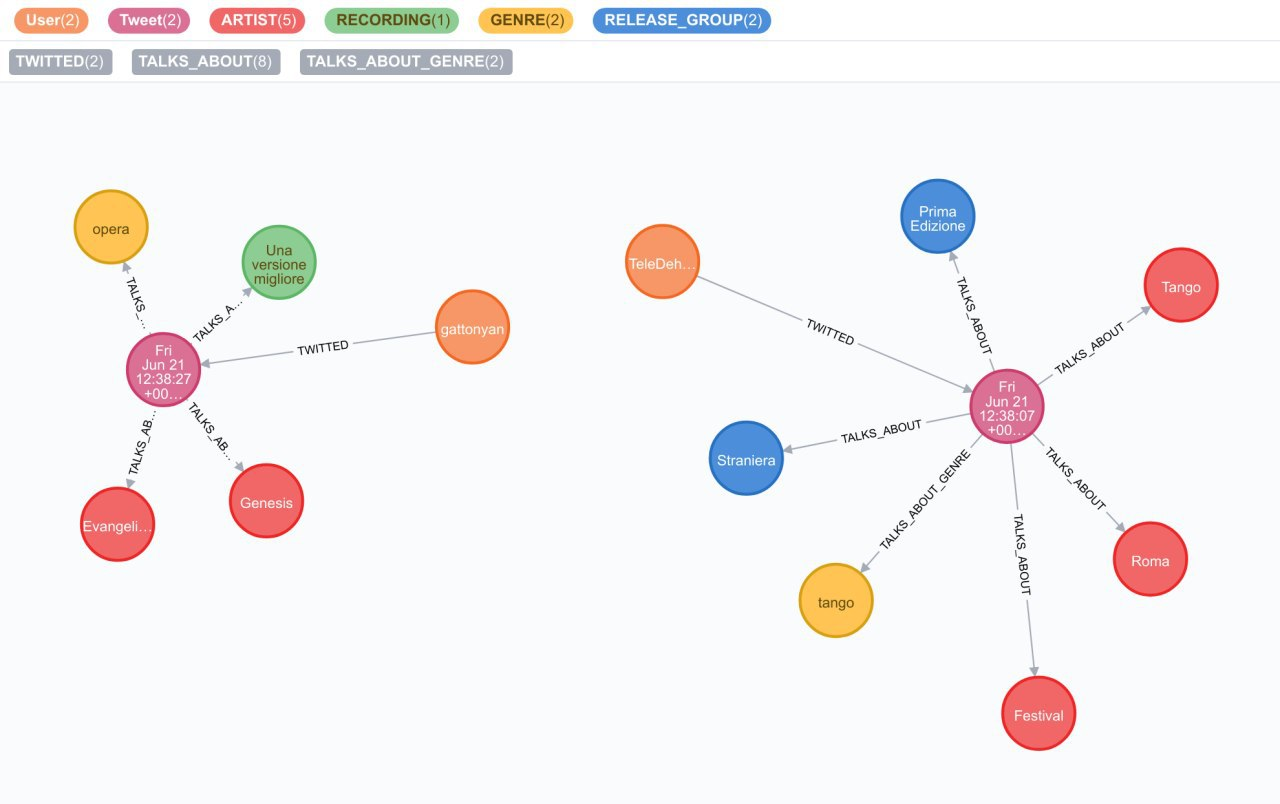
\includegraphics[width=0.8\linewidth]{small_graph.png}
  \caption{Configurazione della struttura del grafo.}
  \label{fig:neo4jmicro}
\end{figure*}

\begin{figure*}[h!]
  \centering
  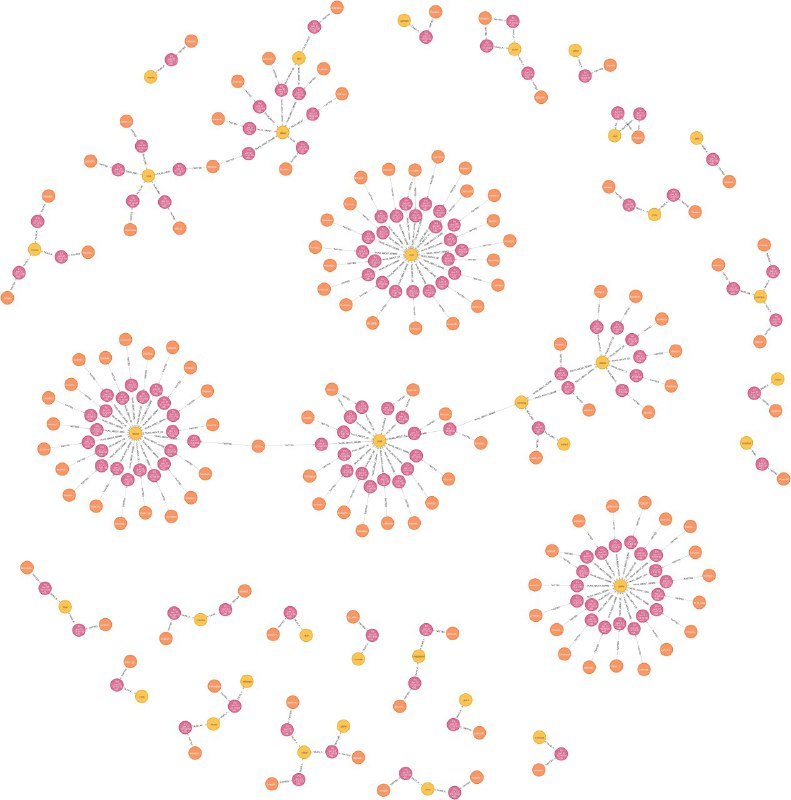
\includegraphics{big_graph.png}
  \caption{Composizione parziale delle comunità all'interno del grafo.}
  \label{fig:neo4jmacro}
\end{figure*}

\section{Riconoscimento delle istanze nel testo}
Data la quantità e qualità dei dati, si è deciso di costruire un strumento di \textit{instance matching} creato \textit{ad hoc} per i tweet: le API disponibili basate su \textit{deep learning} sono spesso allenate su altri tipi di testo (articoli di giornale o opere letterarie) e spesso non offrono una velocità adeguata per l'analisi in tempo reale.
Il problema della qualità del testo è fondamentale: serve uno strumento che riesca ad analizzare il testo e a trovare le entità corrispondenti senza bisogno di contestualizzazione.
Per tale scopo, filtrati già in partenza i tweet grazie a parole chiave a tema musicale, si costruisce un modello che identifichi le istanze restituendone gli \verb|id| grazie all'API di musicbrainz disponibile per Python.

\subsection{Identificazione delle entità}
Le entità sono riconosciute non mediante \textit{machine learning} ma grazie a semplici stratagemmi linguistici e l'aiuto di un correttore ortografico.
Prima di tutto il testo del tweet è ripulito da eventuali abbreviazioni gergali (che vengono sostituite dalla propria forma estesa), link e caratteri speciali.
Subito dopo sono ricercate le parole nel testo che non risultano essere italiane: analizzando tweet in lingua italiana, il cui tema è sicuramente musicale, si presume che una stringa in lingua diversa abbia una certa importanza; ciò è fatto sia analizzandone l'ortografia sia verificando con un'espressione regolare che le parole rispecchino la regola di costruzione delle sillabe in italiano\footnote{Una sillaba in italiano è composta da un massimo di tre consonanti iniziali, vocale ed eventuale consonante finale.}.
In tal caso, o la parola è un sostantivo della quinta classe (parole straniere entrate nell'uso comune) o un termine in lingua non italiana e quindi degno di attenzione.
Infine sono analizzate le parole la cui iniziale è maiuscola, col supporto di un albero sintattico (costruito grazie ad un programma estero, \verb|TreeTagger|\footnote{\url{https://www.cis.uni-muenchen.de/~schmid/tools/TreeTagger/}}, interfacciato con Python grazie ad un wrapper\footnote{\url{https://perso.limsi.fr/pointal/doku.php?id=dev:treetaggerwrapper}} fornito dagli stessi sviluppatori) per verificare che siano nomi propri.

Grazie all'uso della punteggiatura e delle preposizioni, si tenta di stabilire se la presunta entità è un artista o un'opera, verificando poi con certezza confrontando con lo \textit{knowledge graph}. \newline

Tramite le API di musicbrainz, attraverso una serie di funzioni \verb|search| è possibile consultare il database sfruttando un server di ricerca costruito utilizzando la tecnologia \textit{Lucene}.
Analizzate le entità e tentato di stabilire cosa rappresentino, si interroga la base di conoscenza con le funzioni \verb|search_artists| e \verb|search_recordings| per le entità riconosciute rispettivamente come artisti e opere, a cui si aggiunge \verb|search_release_groups| (funzione relativa alla ricerca degli album), per quelle di tipologia incerta.
Per verificare la corrispondenza tra entità e risultati di ricerca, si è scelta la politica di accettare il risultato la cui similarità coseno è maggiore, a patto che superi una soglia arbitraria di $0.95$.
Inoltre, per aumentare la precisione, si sono incrociati i risultati parziali delle ricerche per testare se nello stesso testo compaia l'opera accompagnata dal proprio autore.

\subsection{Prestazioni del modello e margini di miglioramento}
La problematica principale emersa nella costruzione del modello è stata la corretta attribuzione dell'entità nei casi di omonimia: questi casi infatti sono molto frequenti tra canzoni ed album relativi ad artisti differenti ed è quindi possibile che il risultato ottenuto non sia quello desiderato.

Inoltre, nonostante il modello offra una buona \textit{performance} nella selezione dei testi riferiti al mondo musicale e nel riconoscimento delle istanze nel testo, continua a presentare alcune imperfezioni.
Un primo difetto deriva dalla difficoltà nella gestione dei casi polisemici: alcuni nomi di genere (in particolare \textit{drone}, \textit{dance}, \textit{club} e \textit{opera}) sono polisemici, distorcendo i valori dell'analisi.
Il programma utilizzato è troppo rudimentale per distinguere il contesto e quindi mostra numerosi falsi positivi: il termine \textit{club} in particolare viene spesso citato all'interno di testi riguardanti qualsiasi tipo di associazione; la parola \textit{drone}, come già accennato nell'introduzione, indica, nella maggior parte dei casi, l'aeromobile; l'espressione "dance" è frequentemente slegata alla musica e \textit{opera} possiede troppi significati per poterli elencare.

Un'altra problematica, non legata al modello ma a \verb|tweepy| è sorta dopo aver rilevato alcuni \textit{tweet} in lingua straniera (perlopiù spagnola) che citavano il termine \textit{trap} senza riferirsi al genere musicale.

Pertanto, il modello raggiunge buoni risultati nell'ambito di tale progetto, rendendo comunque necessari ulteriori tentativi di miglioramento della sua capacità di riconoscere il contesto all'interno del quale le parole vengono citate.

\hfill
\newpage
\part{Visualizzazioni dei dati}


\hfill
\newpage
\part{Risultati e conclusioni}
% Quanti tweet abbiamo raccolto? Cosa abbiamo osservato? Quali dinamiche esistono tra le comunità e quali sono quelle più grandi?
Nel breve periodo in cui la macchina virtuale è rimasta online a raccogliere i \textit{tweets}, sono stati raccolti 



%----------------------------------------------------------------------------------------
%	BIBLIOGRAPHY
%----------------------------------------------------------------------------------------

\hfill
\newpage
\printbibliography[title={Bibliografia e sitografia}]

%----------------------------------------------------------------------------------------

\end{document}
